\section{Methods}
\label{methods}
%From ILO:
%"Plan and carry out a small-scale investigation of an algorithmic research problem. This investigation could be theoretical, experimental, or both."
This section will cover the methods used throughout the project for conducting the experiments and reaching the goals reported in later sections. An implementation of \qs{} is found on a GitHub repository by Tal Wagner\footnote{https://github.com/talwagner/quadsketch}(one of the authors of \cite{wagner17}) accompanied by SIFT, MNIST, and a "glove" dataset. As such, the NYC Taxi and Diagonal datasets are not included, although they use these in their experiments. This repository has been forked on GitHub and used for carrying out experiments\footnote{https://github.com/aelillie/quadsketch}. As the experiments also require a baseline comparison algorithm, a version of what they describe as "Grid" has been implemented. The methods used for the verification process are described in \ref{experiment_verification}. Furthermore a synthetic dataset has been generated for experimenting with the \qsr{} contribution. The methods used in these experiments are described in \ref{possible_improvements}.  
%The motivation behind each method is to support the problem definition and the analysis of the \qs{} implementation. The analysis consists of verifying the correctness of the stated results and applying the implementation with other data inputs to verify the relation between \qs{} and the baseline. Furthermore a number of practical tests are conducted to research possible performance gains.

\subsection{Experiment verification}
\label{experiment_verification}
Section \ref{baseline} describes the "Grid" baseline implementation, and its role in the experiments, while \ref{datasets} introduces the datasets used in the experiments.

\subsubsection{Baseline comparison: \gr{}}
\label{baseline}
The paper compares the \qs{} performance with other compression algorithms, including (\pq{}) and a simple baseline algorithm, \gr{}. In order to properly assess the quality of the results for the \qs{} and \qsr{} algorithms, a version of Grid has been implemented in \texttt{grid.cpp} as baseline to use for replication experiments. The basic concept is to make a number of \textit{landmarks} equally distributed over the range of each dimension in the dataset. In the compression scheme, each point will for each dimension have its value rounded to the nearest landmark. By doing so, the value of the point is represented by $\log_2(l)$ bits, where $l$ is the number of landmarks used. A simple illustration of this is presented in figure \ref{landmarks}. The horizontal line represent a range of values from 1.0 to 2.0 in one dimension with six points (the colored lines). Above the horizontal line four landmarks are placed, which are represented with 2 bits. In this example the red coordinate(leftmost) would be rounded to 00, the blue and purple(next two) to 01, the green(second from right) to 10, and the yellow(rightmost) to 11.

\begin{figure}[h]
	\centering
	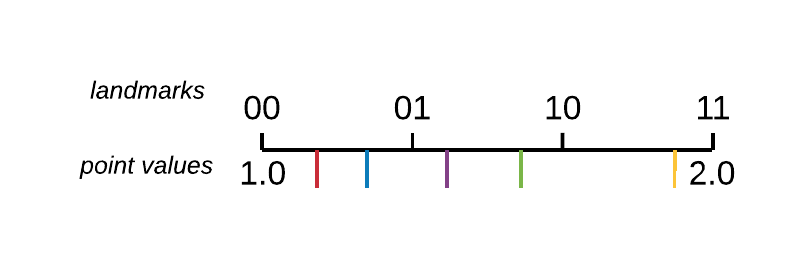
\includegraphics[width=\textwidth]{figures/Landmarks.png}
	\caption{Illustration of \gr{} in one dimension}
	\label{landmarks}
\end{figure}

\subsubsection{Selected Datasets}
\label{datasets}
To ensure proper verification of the results for the \qs{}, the implementation and baseline is tested on two of the datasets used reported in the paper, namely SIFT and MNIST, as these were already available from their repository. Furthermore a synthetic dataset has been generated, both to test \qs{} on a different kind of dataset, but also for experimental reasons for \qsr{}, which is elaborated on in section \ref{clusters}. 
\\
Lastly \qs{} is tested on the GIST dataset. %GIST uses global descriptors, and similarly to the smaller SIFT dataset which uses local descriptors, the idea is to use set of perceptual dimensions  such as naturalness, openness, roughness, expansion, ruggedness. These perceptual dimensions represent the dominant spatial structure of a scene \cite{MattD}. 
GIST is an interesting dataset to consider, as it has a high number of dimensions and a high aspect ratio, and it is used to test the performance of \pq{} in \cite{schmid9} but not used in \cite{wagner17} where the performance of \qs{} is compared to \pq{}. If the results from the experiments turn out to be equivalent or close to the results given in \cite{wagner17}, it will strengthen the credibility of the practical efficiency of \qs{}. 
\\
\\
Applying \qs{} to other datasets could provide some additional insight into how the properties of the datasets might impact the resulting sketch. These results could then be used to e.g. derive heuristics for \qs{} or set a standard for which parameters \qs{} should use. This is further discussed in section \ref{futurework}.

The properties of the datasets used for verification, as well as for experiments, are summarized in table \ref{tab:datasets}.

\begin{table}[h]
	\centering
	\begin{tabular}{l l l l}
		\hline
		Dataset & Points & Dimensions & Aspect ratio ($\Phi$) \\
		\hline
		\sift{} & 1,000,000 & 128 & $\geq$ 83.2 \\
		\mnist{} & 60,000 & 784 & $\geq$ 9.2 \\
		\clust{} & 1,000,000 & 128 & 57.9 \\
		\gist{} & 1,000,000 & 960 & $\geq$ 580 \\
		\hline
	\end{tabular}
	\caption{Properties of the datasets}
	\label{tab:datasets}
\end{table}

\subsection{Experimenting with possible improvements}
\label{possible_improvements}
A number of experiments have been conducted in an attempt to improve \qs{}. The approaches and experiments will be elaborated on below.

\subsubsection{Finding improvements}
\label{finding_improvements}
The paper under investigation, \cite{wagner17}, together with their implementation, \texttt{qs.cpp}, has been thoroughly studied in order to find possible practical improvements to their algorithm. An interesting property was the replacement of "non-important" bits with just zeros. Looking through the source code it appears as if a sketch is not build per se. Instead the \qt{} data structure is built, including the pruning step, where they omit adding bits to represent a node, if it is on a \textit{long edge} path in the tree, i.e. a node whose bits omission would have little effect on the approximation quality\cite[p. 3, l. 14]{wagner17}. They do this on lines 73-76, where they check the condition for pruning, and if it is satisfied they continue, otherwise they add a bit. The code is extracted and illustrated in listing \ref{lst:qs} below:

\begin{lstlisting}[caption={Pruning},label={lst:qs}]
if (long_edge_length >= lambda && parts.size() == 1) {
	continue;
}
new_p[j] += 1.0 / (2.0 * (1 << depth));
\end{lstlisting}

Experimenting with this code allowed for comparing the results to \qs{} and observe if it yielded any results. The implementation is described in \ref{qsr}.


\subsubsection{Synthetic dataset: \clust{}}
\label{clusters}
A synthetic dataset has been generated, with the goal to illustrate a scenario where \qsr{} in practice \textit{should} perform better than \qs{}. It is called \clust{}, as it contains four clusters of rather dense data points in Euclidean space. The clusters' centroids are programmed to be in each "corner" of the dataset(i.e. far apart). A simple illustration of this is presented in figure \ref{fig:clusters}, showing four clusters with each three points in 2D space.

\begin{figure}[h]
	\centering
	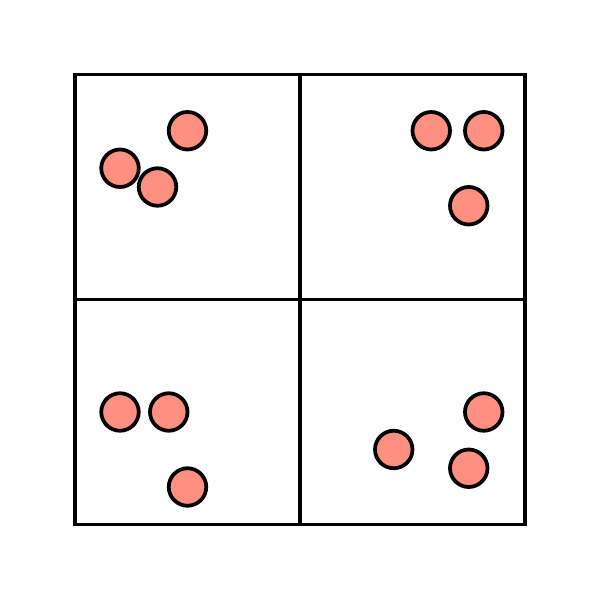
\includegraphics[scale=0.5]{figures/Clusters_example.png}
	\caption{Example of \clust{} in 2D space}
	\label{fig:clusters}
\end{figure}


\texttt{gen.cpp} is implemented to generate a dataset with such four clusters, taking as parameters the number of points, dimensions, and queries, as well as the minimum and maximum value in the dataset(which is the main factor for the resulting aspect ratio). The C++ library \texttt{normal\_distribution}\footnote{http://www.cplusplus.com/reference/random/normal\_distribution/} is used to randomly distribute the points in a cluster according to a \textit{normal distribution}, defined by a mean ($\mu$) with a specific standard deviation ($\sigma$). 

The generated set used for testing has 1,000,000 points, 128 dimensions and a resulting aspect ratio ($\Phi$) of 57.9, obtained from a minimum value of 100 and a maximum value of 600. 10,000 points (1\% of the dataset) are extracted to make up the query points. \clust{} are generated from two \texttt{normal\_distribution} generators fed with mean values of 162.5 and 537.5 respectively, and both with a standard deviation of 62.5. The properties of the dataset are also summarized in table \ref{tab:datasets}.